\documentclass[11pt,a4paper]{article}

\usepackage[utf8]{inputenc}
\usepackage[T1]{fontenc}
\usepackage[margin=1in]{geometry}
\usepackage{amsmath}
\usepackage{booktabs}
\usepackage{float}
\usepackage{graphicx}
\usepackage{hyperref}
\usepackage{enumitem}
\usepackage{tabularx}
\usepackage{xcolor}

\graphicspath{{../}}
\setlength{\emergencystretch}{3em}
\hypersetup{
    colorlinks=true,
    linkcolor=blue!50!black,
    citecolor=blue!50!black,
    urlcolor=blue!50!black
}

\title{Generative Image Modelling on Cat Images}
\author{Mateusz Iwaniuk \and Adam Kaniasty}
\date{June 2026}

\begin{document}

\maketitle

\begin{abstract}
This report summarizes a project on lightweight generative modelling for cat images.
The main comparison covers DCGAN, adversarial autoencoder (AAE), and VQ-VAE models trained from scratch under a constrained compute budget.
The primary metric is Frechet Inception Distance (FID), supported by generated sample grids, latent interpolation, simple image-quality diagnostics, and training curves.
The strongest result is obtained by DCGAN at $128\times128$ resolution with FID $232.964$.
The main limitations are limited repeated experiments, limited hyperparameter optimization, heuristic checkpoint interpretation for GAN training, and dependence on FID as the main quantitative metric.
\end{abstract}

\tableofcontents
\newpage

\section{Introduction and Research Question}

The goal of this project was to compare several lightweight generative modelling approaches on the task of cat image generation. The central question was which model family gives the best practical trade-off between visual quality, diversity, training stability, and computational cost under the constraints of the course project.

The comparison covers three model families: DCGAN, adversarial autoencoder (AAE), and VQ-VAE. The models are evaluated using Frechet Inception Distance (FID), generated sample grids, simple image-quality diagnostics, learning curves, and latent interpolation for models with continuous latent spaces. As an exploratory extension, the best-performing model family was also trained on a mixed cats-and-dogs subset.

\section{Theoretical Background and Literature Review}

\subsection{Generative Adversarial Networks and DCGAN}

Generative adversarial networks train two models in a minimax game: a generator and a discriminator \cite{goodfellow2014gan}. The generator maps random latent vectors to images, while the discriminator learns to distinguish generated images from real training images. DCGAN adapts this idea to convolutional image generation and is commonly used as a lightweight baseline for image synthesis tasks \cite{radford2015dcgan}.

DCGAN is relevant here because adversarial training can produce sharper samples than reconstruction-based autoencoders. At the same time, GAN training is unstable and sensitive to optimizer settings. In this project, the main DCGAN risks were:

\begin{itemize}[leftmargin=*]
    \item discriminator overpowering the generator;
    \item mode collapse or reduced sample diversity;
    \item sensitivity to generator/discriminator learning-rate balance;
    \item difficulty choosing checkpoints from loss curves alone.
\end{itemize}

\subsection{Adversarial Autoencoders}

An adversarial autoencoder combines an autoencoder reconstruction objective with adversarial regularization of the latent space \cite{makhzani2015aae}. The encoder and decoder learn to reconstruct images, while a latent discriminator encourages encoded samples to match a chosen prior distribution. This gives the model a continuous latent space that can be sampled and interpolated.

For this project, the AAE is useful as a contrast to DCGAN: it has a more explicit reconstruction objective and smoother latent structure, but it is expected to produce blurrier images. The main risk is that the adversarial latent constraint does not guarantee realistic decoded samples.

\subsection{VQ-VAE}

VQ-VAE uses discrete vector-quantized latent codes instead of a continuous Gaussian latent representation \cite{oord2017vqvae}. The encoder output is mapped to entries from a learned codebook, and the decoder reconstructs the image from the selected discrete codes.

Generation with VQ-VAE requires a sampling strategy over the discrete latent codes. In this implementation, generated samples are produced using empirical code frequencies rather than a separately trained autoregressive prior. This makes the model simpler, but it can limit sample diversity because spatial structure in the latent codes is not explicitly modelled.

\subsection{FID and Qualitative Evaluation}

FID compares generated and real image distributions in an Inception feature space \cite{heusel2017fid}. Lower FID usually indicates that generated images are closer to the reference distribution. However, FID depends on image resolution, preprocessing, reference split, and sample count, so scores from the 64x64 and 128x128 phases should not be treated as directly comparable.

FID is useful but incomplete. A low score does not guarantee that samples are visually convincing, and it may miss failures such as local artifacts or semantic ambiguity. For this reason, FID is combined with sample grids, learning curves, latent interpolation, and simple diagnostic statistics.

\section{Dataset and Preprocessing}

The main dataset is the Kaggle Cat Dataset, which contains approximately ten thousand cat images \cite{kagglecats}. The exploratory mixed-domain extension uses images from the Kaggle Dogs vs. Cats dataset \cite{kaggledogsvscats}.

The experiments use two evaluation settings:

\begin{itemize}[leftmargin=*]
    \item a smaller 64x64 cluster sweep with 1500 training cats and 500 FID reference cats;
    \item a full 128x128 phase with 3000 training cats and 1000 FID reference cats.
\end{itemize}

Images are converted to RGB, resized or cropped to the target resolution, normalized to $[-1,1]$, and horizontally flipped during training. Because the phases use different resolutions and sometimes different split sizes, 64x64 and 128x128 FID values should be interpreted separately.

\begin{figure}[H]
    \centering
    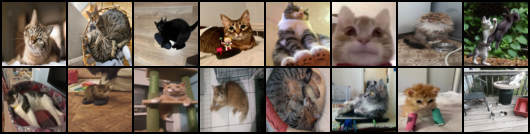
\includegraphics[width=0.75\textwidth]{presentation/assets/dataset/dataset_preview.png}
    \caption{Preprocessed cat training examples.}
    \label{fig:dataset-preview}
\end{figure}

\section{Models and Training Pipeline}

\begin{table}[H]
\centering
\caption{Main model families.}
\begin{tabularx}{\textwidth}{@{}lXrr@{}}
\toprule
Model & Main idea & 64x64 params & 128x128 params \\
\midrule
DCGAN & Generator and discriminator trained adversarially & 5.4M & 9.6M \\
AAE & Autoencoder plus adversarial latent regularizer & 7.7M & 12.0M \\
VQ-VAE & Autoencoder with discrete vector-quantized latent codebook & 0.5M & 1.0M \\
\bottomrule
\end{tabularx}
\end{table}

The implementation uses PyTorch Lightning. Each run is identified by a reproducible \texttt{run\_id} derived from the model, configuration hash, and seed. Runs write manifests, metrics CSV files, events JSONL files, sample grids, checkpoints, FID JSON files, quality JSON files, learning curves, and interpolation figures where applicable.

The checkpointing policy differs by model family. The training script saves \texttt{last.ckpt}. Some DCGAN configurations also set \texttt{save\_every: 5} for periodic checkpointing. AAE and VQ-VAE configurations include early stopping on reconstruction loss. DCGAN runs do not use standard early stopping because GAN losses are not reliable validation objectives; instead, they are evaluated using FID, samples, and learning curves after training.

\section{Hyperparameter Optimization and Experiment Design}

The hyperparameter search was intentionally limited. It should be understood as a small sweep and targeted refinement process, not as exhaustive optimization. This is important when interpreting the results, because a better configuration may exist outside the tested grid.

\begin{itemize}[leftmargin=*]
    \item DCGAN variants changed latent dimension, learning rate, batch size, generator design, label smoothing, and generator/discriminator learning-rate balance.
    \item AAE variants changed latent dimension, learning rate, batch size, and image size.
    \item VQ-VAE variants changed codebook size, embedding dimension, learning rate, batch size, and image size.
\end{itemize}

The experiment set contains multiple runs, but most of them correspond to different hyperparameter settings or experimental phases. They are not independent repeated trials with different random seeds. For that reason, model-level means and standard deviations across repeated training runs are not claimed. Per-image or per-pair statistics are reported where available.

\section{Experiments}

\subsection{Part A: 64x64 Sweep and Refinement}

Part A was an initial comparison of DCGAN, AAE, and VQ-VAE under a smaller compute setting. It used 1500 training cat images and 500 FID reference images at 64x64 resolution.

In this phase, DCGAN achieved the lowest FID among the three representative refined runs. However, the generated samples remained visually weak, with many blob-like textures and incomplete cat shapes. The refinement stage improved the comparison setup, but it did not solve the semantic image-quality problem.

\begin{table}[H]
\centering
\caption{Representative 64x64 refined results.}
\begin{tabular}{@{}llr@{}}
\toprule
Model & Run & FID \\
\midrule
DCGAN & \texttt{dcgan\_5150b7dc\_42} & 287.0 \\
AAE & \texttt{aae\_b2d7b809\_42} & 306.5 \\
VQ-VAE & \texttt{vqvae\_fdb2d5a9\_42} & 421.0 \\
\bottomrule
\end{tabular}
\end{table}

\begin{figure}[H]
    \centering
    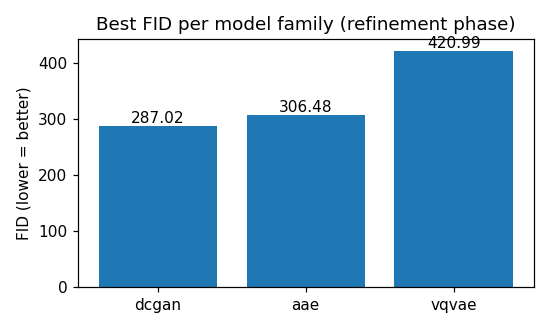
\includegraphics[width=0.78\textwidth]{presentation/assets/part64/fid_bar.png}
    \caption{64x64 FID comparison. Lower is better.}
    \label{fig:part64-fid}
\end{figure}

\begin{figure}[H]
    \centering
    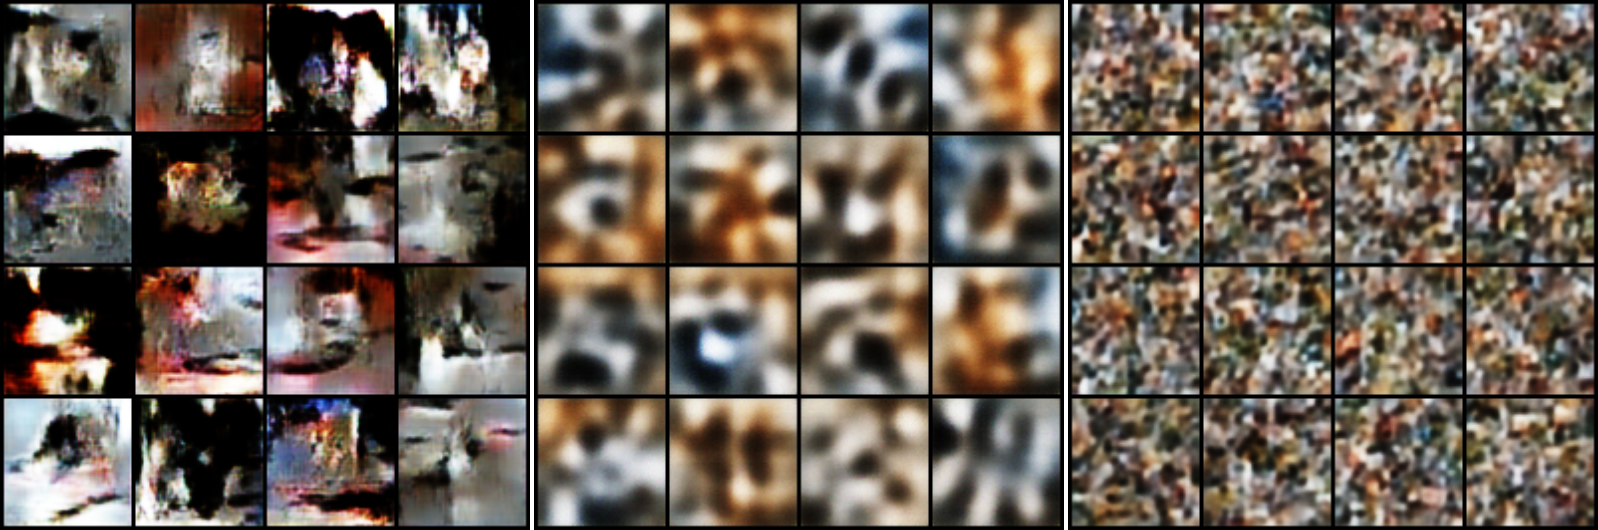
\includegraphics[width=\textwidth]{presentation/assets/part64/compare_grid.png}
    \caption{64x64 generated sample grids for DCGAN, AAE, and VQ-VAE.}
    \label{fig:part64-grid}
\end{figure}

\subsection{Part B: 128x128 Main Comparison}

Part B repeated the model comparison at 128x128 resolution using the full planned cat split: 3000 training cats and 1000 reference cats. This phase gives the main result of the project.

DCGAN achieved the best FID, followed by AAE. The representative 128x128 VQ-VAE run had the worst FID among the three model-family representatives under the implemented empirical-code sampling procedure. Visually, DCGAN samples contained more recognizable cat-like fragments than the AAE samples, although they still contained substantial artifacts. DCGAN also had a higher diversity statistic than both AAE and VQ-VAE in \texttt{quality.json}.

\begin{table}[H]
\centering
\caption{Main 128x128 results.}
\resizebox{\textwidth}{!}{%
\begin{tabular}{@{}llrrrr@{}}
\toprule
Model & Run & FID & Sharpness sample mean $\pm$ std & Diversity sample mean $\pm$ std & NN mean \\
\midrule
DCGAN & \texttt{dcgan\_e9574605\_42} & 232.964 & $0.0169 \pm 0.0083$ & $18.493 \pm 1.736$ & 17.062 \\
AAE & \texttt{aae\_7ad02727\_42} & 289.050 & $0.0087 \pm 0.0024$ & $16.075 \pm 2.154$ & 16.962 \\
VQ-VAE & \texttt{vqvae\_28e76f2a\_42} & 489.819 & $0.0178 \pm 0.0010$ & $9.590 \pm 1.800$ & 17.245 \\
\bottomrule
\end{tabular}
}
\vspace{0.3em}

\footnotesize{Sharpness, diversity, and nearest-neighbor diagnostics are single-run statistics from \texttt{eval/quality.json}. The standard deviations are over generated samples or pairwise feature distances, not over repeated random seeds.}
\end{table}

\begin{figure}[H]
    \centering
    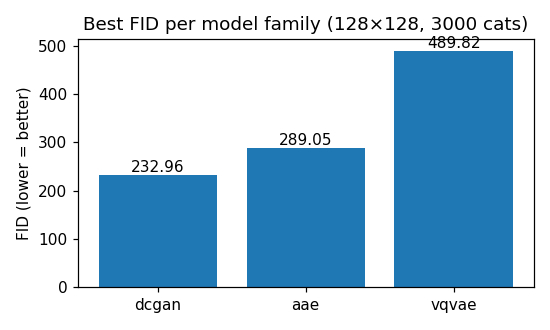
\includegraphics[width=0.78\textwidth]{presentation/assets/part128/fid_bar.png}
    \caption{128x128 FID comparison.}
    \label{fig:part128-fid}
\end{figure}

\begin{figure}[H]
    \centering
    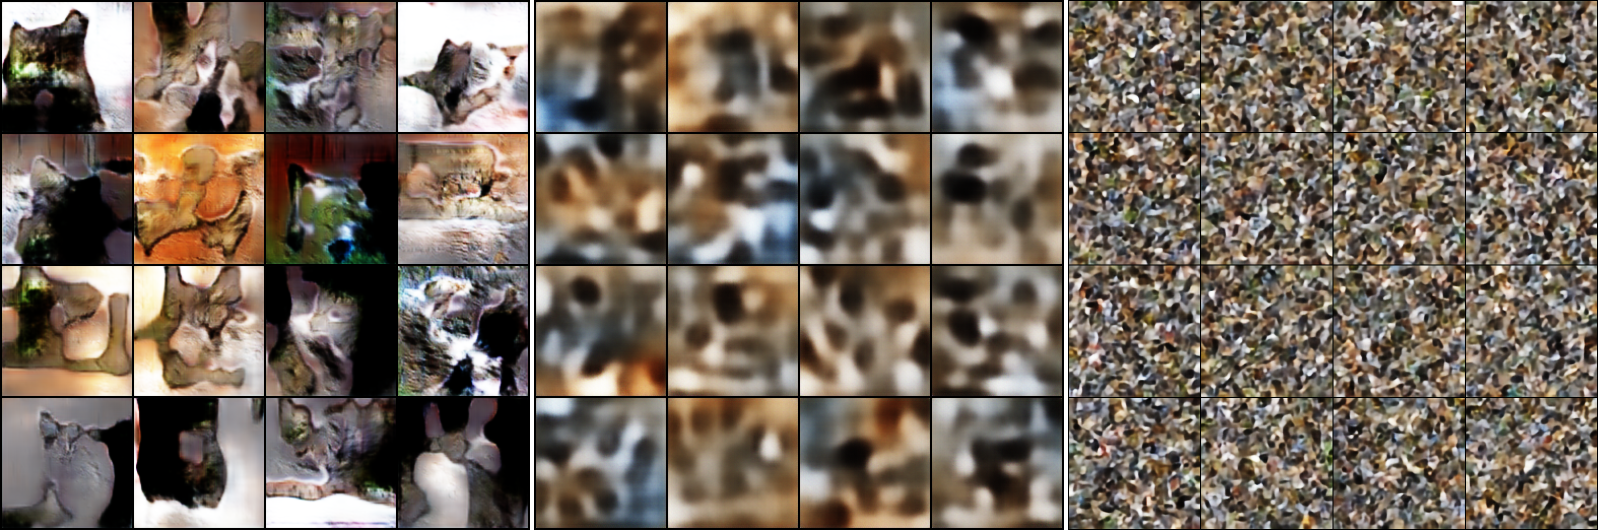
\includegraphics[width=\textwidth]{presentation/assets/part128/compare_grid.png}
    \caption{128x128 generated sample grids for DCGAN, AAE, and VQ-VAE.}
    \label{fig:part128-grid}
\end{figure}

\subsection{Part C: DCGAN Generator/Discriminator Rebalance}

Part C tested whether rebalancing the DCGAN generator and discriminator would improve the best 128x128 result. This was motivated by the Phase B DCGAN learning curves, where the generator loss plateaued and the discriminator appeared relatively strong.

The rebalance changed three settings:

\begin{itemize}[leftmargin=*]
    \item generator learning rate increased from $10^{-4}$ to $2\cdot10^{-4}$;
    \item discriminator learning rate decreased from $2\cdot10^{-4}$ to $10^{-4}$;
    \item label smoothing decreased from $0.1$ to $0.05$.
\end{itemize}

The modification did not improve the result. FID worsened from 232.964 to 243.147, so the original Phase B DCGAN remains the best run.

\begin{table}[H]
\centering
\caption{DCGAN Phase B baseline versus Part C rebalance.}
\begin{tabular}{@{}lrrrr@{}}
\toprule
Run & FID & Sharpness sample mean $\pm$ std & Diversity sample mean $\pm$ std & NN mean \\
\midrule
\texttt{dcgan\_e9574605\_42} & 232.964 & $0.0169 \pm 0.0083$ & $18.493 \pm 1.736$ & 17.062 \\
\texttt{dcgan\_30f57e20\_42} & 243.147 & $0.0157 \pm 0.0076$ & $18.650 \pm 1.810$ & 17.501 \\
\bottomrule
\end{tabular}
\vspace{0.3em}

\footnotesize{Quality diagnostics are single-run statistics from \texttt{eval/quality.json}; the standard deviations are not repeated-seed statistics.}
\end{table}

\begin{figure}[H]
    \centering
    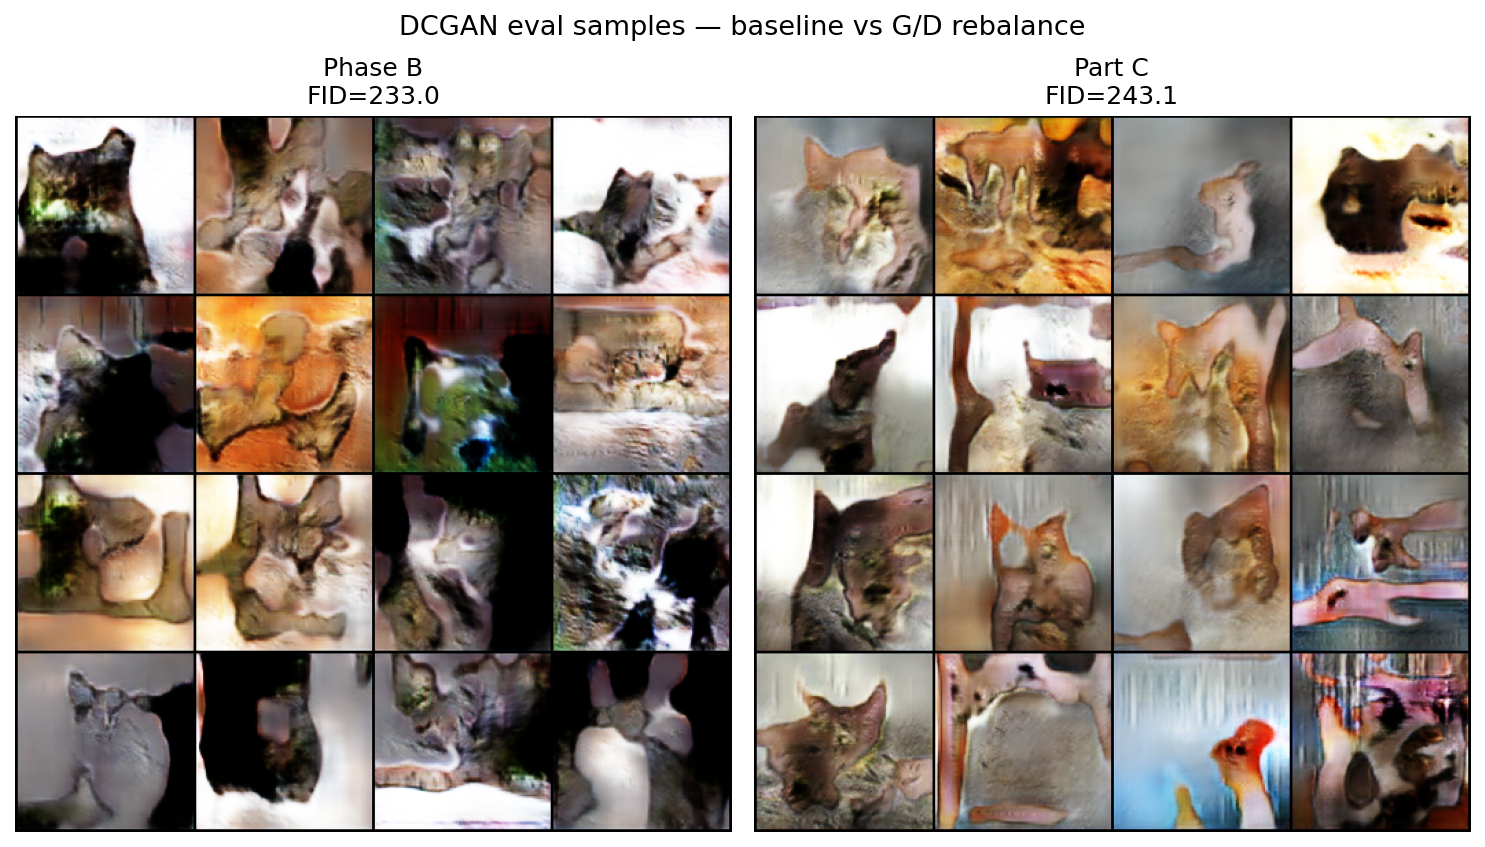
\includegraphics[width=\textwidth]{presentation/assets/partc/gd_compare.png}
    \caption{Phase B DCGAN baseline versus Part C rebalance sample comparison.}
    \label{fig:partc-gd}
\end{figure}

\subsection{Cats-and-Dogs Extension}

The mixed cats-and-dogs extension used DCGAN because it was the best-performing model family in the cats-only comparison. The goal was exploratory: to test whether the same unconditional architecture could model a broader visual distribution without class conditioning.

The 128x128 mixed run reached FID around 271 against the mixed reference split. Because the model is unconditional, generated outputs can become ambiguous mixtures of cat-like and dog-like visual features rather than clearly separated classes.

\begin{figure}[H]
    \centering
    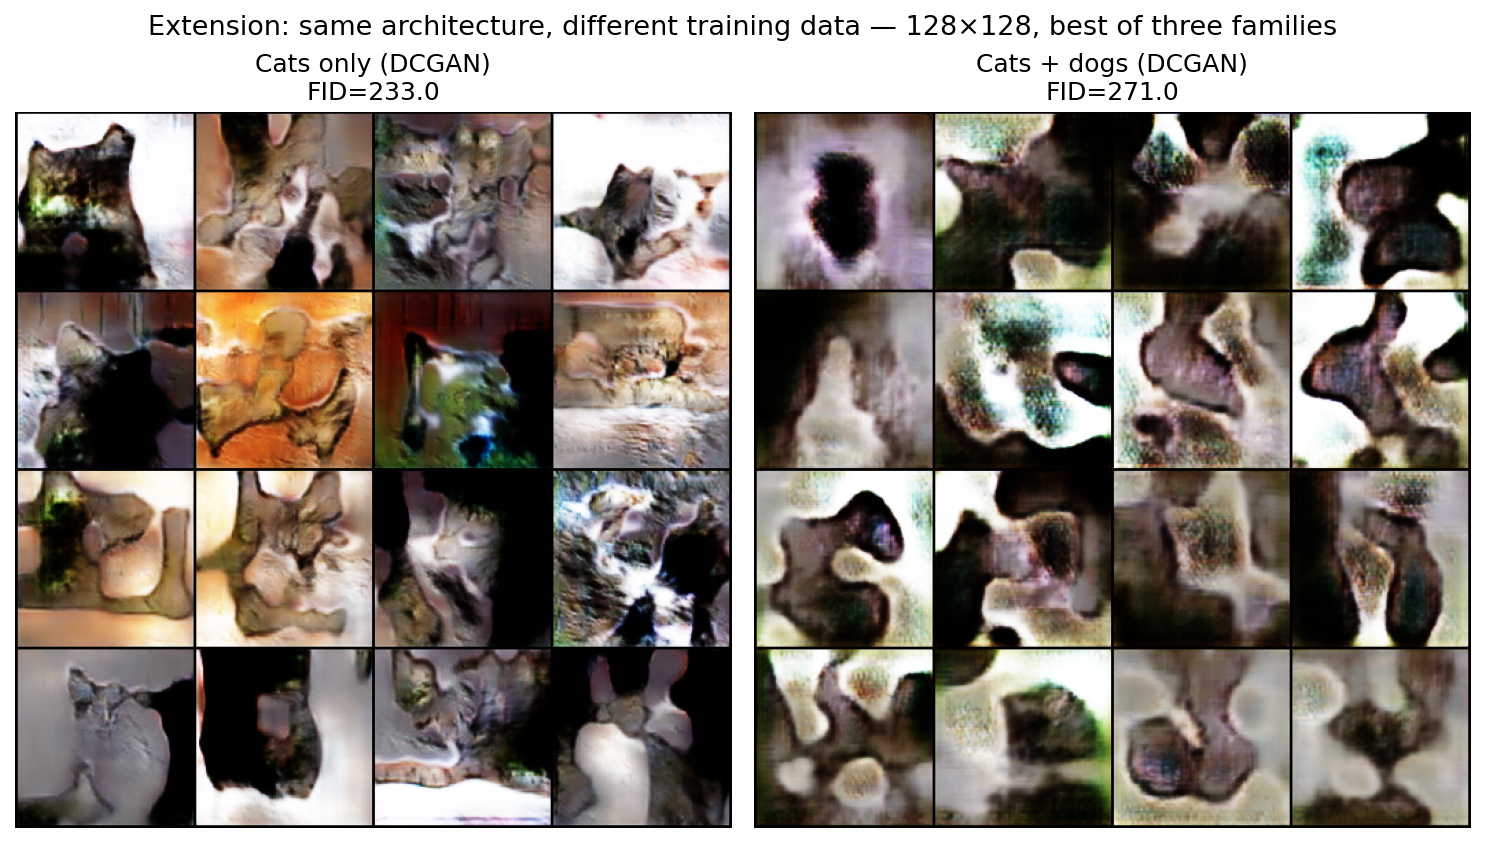
\includegraphics[width=\textwidth]{presentation/assets/part128/ext_compare.png}
    \caption{Cats-only versus mixed cats-and-dogs DCGAN sample comparison.}
    \label{fig:extension}
\end{figure}

\section{Learning Curves and Checkpoint Analysis}

Learning curves are included because they show training dynamics that are not visible from final FID alone.

For DCGAN, the curves track generator loss, discriminator loss, and sample standard deviation. For AAE, they track reconstruction loss, adversarial generator loss, adversarial discriminator loss, and sample standard deviation. For VQ-VAE, they track reconstruction loss, commitment loss, perplexity, and codebook usage statistics.

The final reported FID values use the completed evaluations. AAE and VQ-VAE use reconstruction-based early stopping configs, while DCGAN uses fixed epochs and post-training evaluation because GAN loss alone is not a reliable early-stopping criterion.

\begin{figure}[H]
    \centering
    \includegraphics[width=0.86\textwidth]{runs/dcgan_e9574605_42/eval/curves.png}
    \caption{Learning curves for the best 128x128 DCGAN run.}
    \label{fig:curves-dcgan}
\end{figure}

\begin{figure}[H]
    \centering
    \includegraphics[width=0.86\textwidth]{runs/aae_7ad02727_42/eval/curves.png}
    \caption{Learning curves for the 128x128 AAE run.}
    \label{fig:curves-aae}
\end{figure}

\begin{figure}[H]
    \centering
    \includegraphics[width=0.86\textwidth]{runs/vqvae_28e76f2a_42/eval/curves.png}
    \caption{Learning curves for the 128x128 VQ-VAE run.}
    \label{fig:curves-vqvae}
\end{figure}

\section{Qualitative Result Analysis}

The qualitative results are consistent with the quantitative ranking, but they also show that none of the tested models produces fully realistic cat images. DCGAN has the best FID among the completed runs, and the 128x128 sample grid contains more recognizable cat-like fragments than the 64x64 DCGAN grid. Nevertheless, the samples remain far from realistic photographs.

The main visual observations are:

\begin{itemize}[leftmargin=*]
    \item DCGAN samples show distorted faces, inconsistent textures, stretched bodies, and occasional non-cat blob structures.
    \item AAE samples are visibly smoother and blurrier, matching the lower sharpness statistic.
    \item VQ-VAE has the lowest diversity statistic among the 128x128 model-family representatives and the highest FID. The sample grids show repeated or reconstruction-like cat images rather than diverse free samples.
\end{itemize}

The VQ-VAE result is consistent with the limitation of empirical code sampling without a learned prior, but this is an interpretation rather than a direct proof. The interpolation artifacts also support the qualitative analysis: DCGAN interpolation changes texture and color gradually, while AAE interpolation remains very blurred. Interpolation quality should be treated as a diagnostic only, not as a replacement for distribution-level evaluation.

Nearest-neighbor distances do not prove absence of memorization, but they provide a first automated check that generated samples are not trivially identical to the nearest training references.

\begin{figure}[H]
    \centering
    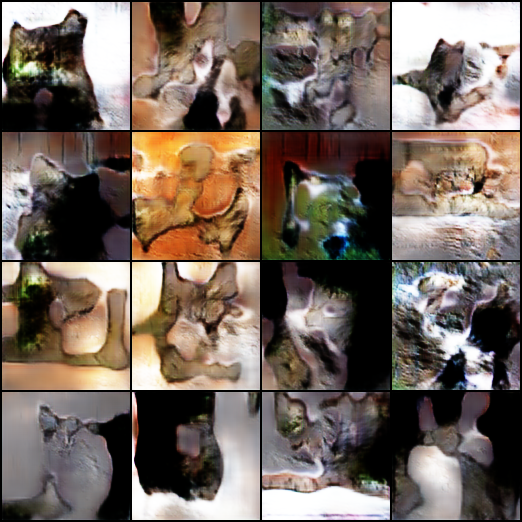
\includegraphics[width=0.86\textwidth]{presentation/assets/part128/hero_dcgan.png}
    \caption{Best 128x128 DCGAN sample panel.}
    \label{fig:hero-dcgan}
\end{figure}

\begin{figure}[H]
    \centering
    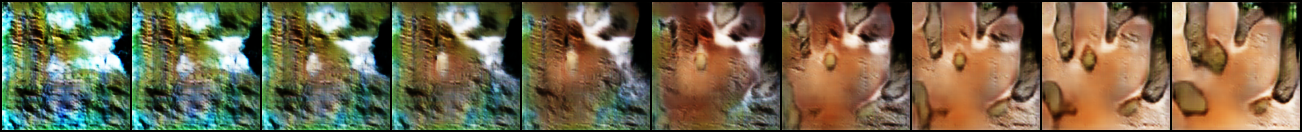
\includegraphics[width=0.86\textwidth]{presentation/assets/part128/interp_dcgan.png}
    \caption{DCGAN latent interpolation at 128x128.}
    \label{fig:interp-dcgan}
\end{figure}

\begin{figure}[H]
    \centering
    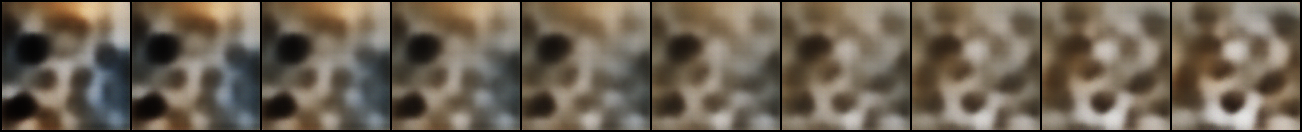
\includegraphics[width=0.86\textwidth]{presentation/assets/part128/interp_aae.png}
    \caption{AAE latent interpolation at 128x128.}
    \label{fig:interp-aae}
\end{figure}

\section{AI Usage Declaration}

AI assistance was used to help draft and organize this report from existing project materials. It was also used to format the LaTeX report structure and bibliography, and during development of scripts for running experiments on the computation cluster.

\section{Limitations}

The main limitation is that the experimental budget was small. Hyperparameter optimization was limited to small sweeps and targeted refinements, and true repeated-seed experiments were not performed. Therefore, the report cannot provide model-level means and standard deviations over independent training repetitions.

The evaluation is also limited. FID is the main quantitative generative metric, and no human evaluation was performed. FID values across 64x64 and 128x128 phases are not directly comparable because the resolution and split sizes differ. VQ-VAE generation is limited by empirical latent-code sampling, so a learned prior may be necessary for a fairer generative evaluation.

Finally, the models are intentionally small. They should be interpreted as lightweight course-project baselines rather than as competitors to high-capacity StyleGAN or diffusion systems. DCGAN early stopping is also not formalized; checkpoint interpretation relies on sample inspection and FID after training.

\section{Conclusions}

Across the completed experiments, DCGAN is the best-performing model family. The 128x128 DCGAN run achieved the best FID, while AAE produced smoother but less realistic samples and VQ-VAE performed poorly under the current empirical-code sampling method. Increasing the resolution and using the full cat split improved the best reported DCGAN result relative to the 64x64 phase.

The G/D rebalance experiment did not improve the best DCGAN run, which suggests that the simple learning-rate and label-smoothing adjustment was insufficient for this setup.

\bibliographystyle{plain}
\bibliography{references}

\end{document}
